\section{Scientific foundations}
\label{sec:foundations}

This section surveys the traditions the methodology lenses (\cref{sec:n3})
are built from, and which part of the system each supports
(\cref{tab:methods}, \cref{fig:lenses}). \evint\ The literature supports the
\emph{constructs} each lens uses: a discrimination, a rival cause, a hedged
rule and its exception, a causal-ambiguity gap. It does not support the
lenses. No study cited here tests whether a detector built on these
constructs finds real expert knowledge in text. That test is what Part III is for.

\begin{figure}[!b]
  \centering
  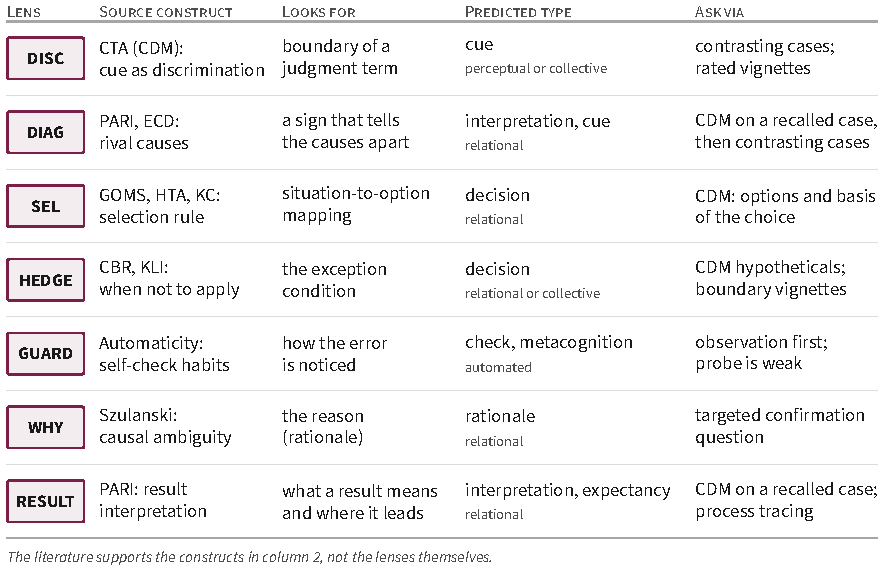
\includegraphics{figures/pdf/fig03_lenses.pdf}
  \caption[Which methodology gives which lens]{Which research method gives
    which methodology lens, and what missing element each lens looks for.
    Every arrow is a construct taken from the literature in this section;
    none of the lenses has been validated against a human judgment of where
    expert knowledge is missing (\cref{tab:methods}).}
  \label{fig:lenses}
\end{figure}

\subsection{Decoding the Disciplines: the bottleneck as framing}

Decoding the Disciplines (DtD) asks instructors to find a bottleneck where many students get stuck.
A ``decoding interview'' uncovers what experts do there; the instructor then models the step, gives
practice and feedback, and assesses it \parencite{middendorf2004decoding,pace2017decoding,pace2021beyond}.
\evlit\ The strongest controlled comparison we found favored DtD on hypotheses, operational
definitions and variables \parencite{pinnow2016decoding}. It covered introductory psychology, with 46
DtD and 45 control students. We found no randomized trial, no
controlled physics study and no retention or transfer measure. \evint\ The bottleneck idea frames which gap-map questions matter for
teaching and, with the model--practice--assess steps, the education path (\cref{sec:education}); the
decoding interview is not used as evidence (\cref{sec:investigated-not-central}).

\subsection{Cognitive task analysis, the Critical Decision Method and PARI}

Cognitive task analysis (CTA) is a family of more than 100 named methods
\parencite{yates2011advancing} for capturing the knowledge, decisions and
cues behind skilled performance
\parencite{schraagen2000cognitive,crandall2006working,clark2008cognitive}.
Its omission numbers are in \cref{sec:problem}. \evlit\ Here what matters is
what CTA-derived knowledge is \emph{worth} once recovered. A
meta-analysis of a small number of studies found CTA-based instruction
outperforms other ways of identifying training content, Hedges'
$g = 0.871$, varying substantially by method and context
\parencite{tofelgrehl2013cognitive}. In surgical training, a 12-study review
found standardized mean differences of 1.36 (95\% confidence interval, CI, 0.67--2.05) for
procedural knowledge and 2.06 (1.17--2.96) for technical performance
\parencite{edwards2021cognitive}. In an undergraduate biology course
(N~=~314, double-blind), CTA-derived instruction cut withdrawal from 8.1\% to
1.4\% of initial enrollment, against an award-winning instructor
\parencite{feldon2010translating}. Interviews with 52 scientists and
engineers yielded 29 problem-solving decisions shared across fields
\parencite{price2021detailed}.

\evint\ The schema's knowledge types (decision, cue, interpretation, check,
expectancy) are CTA categories. Pooling experts recovers more than any one
expert, so future gold standards are a union of experts plus a behavioral
trace. Published CTA task lists are candidate gold for the retrospective
study (\cref{sec:validation}). The thin but positive instructional evidence
is the basis for the education path.

\paragraph{The Critical Decision Method (CDM).} CDM works over one real,
recalled incident in several passes: a timeline, deepening probes, then
``what if'' questions \parencite{hoffman1998use}. It extends the
critical-incident technique with probes for perceptual and conceptual
discriminations, typicality judgments and critical cues
\parencite{klein1989critical}; ACTA is a streamlined practitioner version
\parencite{militello1998applied}. \evint\ CDM's probe for discriminations and typicality is the construct
behind the DISC lens, which fires when sources use a judgment term (``high
risk,'' ``abnormal'') without stating its boundary. CDM's other probes give
the human channel for DIAG, SEL, HEDGE and RESULT. Its question discipline is
the rule every lens's questions follow: retrospective, anchored to a real
incident, no yes/no questions, one construct per question.

\paragraph{PARI.} PARI (Precursor, Action, Result, Interpretation) was built
for U.S. Air Force troubleshooting training. For each step it records why the
action was taken, the action, its result, and what the result means for the
fault hypothesis \parencite{hall1995procedural}. It reports no outcome
statistics. Interpretation is where pooled expert coverage stayed lowest in
the programming study of \cref{sec:problem}. \evint\ PARI's
result-to-interpretation step is the construct behind the RESULT lens, which
fires when sources prescribe a test or check but never say which result maps
to which action. Joined with Evidence-Centered Design's alternative
explanations (below), the same step gives DIAG its construct: rival causes of
one effect with no sign in the text that separates them.

\subsection{Expert--novice differences}

\evlit\ In sorting tasks and think-aloud protocols, experts categorized
physics problems by the principle that solves them and novices by surface
features \parencite{chi1981categorization}. Experts recognize patterns and
chunks that guide them \parencite{larkin1980expert,chase1973perception}.
Perceptual expertise can
be taught directly. In chick sexing, naive participants given a short
instruction on one shape contrast rose from near-chance to expert-level
accuracy. Their item-level agreement with experts rose from a correlation of
.21 to .82 \parencite{biederman1987sexing}. \evint\ A
perceptual cue is therefore a discrimination that contrasting cases can
teach, which is why DISC's human channel routes to contrasting-case
classification and not to interviews alone. The knowledge type
\code{expert_novice_contrast} and the planned bottleneck-hypothesis object
(``expert has, novice lacks, novice substitutes'') come from this work.

\subsection{What experts misjudge about learners}
\label{sec:foundations-learners}

\begin{evlitbox}
  Three blind-spot findings, each at its own grain. Among 48 preservice
  secondary teachers, those with more advanced mathematics
  education were more likely to treat symbolic equations as a prerequisite
  for word and story problems, the reverse of students' actual performance
  pattern \parencite{nathan2003expert}. In two studies, one with expertise
  experimentally manipulated, participants with more expertise predicted
  novice task-completion times worse and resisted debiasing; intermediates
  may be the more accurate predictors \parencite{hinds1999curse}. In a physics study, 25
  first-year physics graduate teaching assistants (TAs) and 30 physics
  instructors predicted introductory students' most common wrong answer on
  each Force Concept Inventory item. The TAs scored 65\% of the maximum
  possible score and the instructors 68\%, against 40\% for random guessing.
  Both groups beat random guessing, and they did not differ significantly
  from each other \parencite{maries2016teaching}.
\end{evlitbox}

\evint\ The pattern recurs across settings, but it is not a general law that
misjudgment grows with expertise. The variable is mathematics coursework in
one study and experimentally induced expertise in another. In the physics
study, the instructors' greater teaching experience did not help. What the findings license is
narrower and sufficient here: expert judgment of learner difficulty is not
reliable evidence of it.

\paragraph{Pedagogical content knowledge (PCK).} Shulman named the knowledge
teachers need beyond subject matter: how to represent a topic, and what
makes it easy or hard for learners, including their preconceptions
\parencite{shulman1986those,shulman1987knowledge}. \evlit\ Across 9,556
students of 181 middle-school teachers, teachers who could identify a popular
wrong answer produced larger gains on the affected items than teachers who
knew only the right answer \parencite{sadler2013influence}. PCK names the
layer the gap map does not reach: knowledge about learners, not about the
domain.

\paragraph{Threshold concepts and conceptual change.} A threshold concept
opens ``a new way'' of seeing a subject and is often ``troublesome'':
counter-intuitive or alien to the learner
\parencite{meyer2003threshold,meyer2005threshold,meyer2006overcoming}; the
framework is conceptual, not an effect size. Research on conceptual change
asks how learners restructure prior ideas. The classical model needs
dissatisfaction and an intelligible, plausible, fruitful replacement
\parencite{posner1982accommodation}. ``Knowledge in pieces'' instead treats
intuitive physics as many small context-bound elements
\parencite{disessa1993toward}, and misconceptions as knowledge in transition
\parencite{smith1994misconceptions}. \evlit\ The Force Concept Inventory
builds its wrong-answer options from common beliefs about force and motion
\parencite{hestenes1992force}, and bug libraries model procedural errors as
systematic ``bugs'' in an otherwise correct procedure
\parencite{brown1978diagnostic}.

\paragraph{What this contributes.} These findings constrain the design. The
GUARD lens never asserts that a learner will find something difficult, only
that sources report guarding against an error. Learner difficulty is a
separate layer, established only from learner response data (concept
inventories are candidate gold in physics); \code{misconception} is stored as
a hypothesis with its evidence, neutral between the classical and
knowledge-in-pieces views. No lens derives from threshold concepts, because
identifying one relies on the expert judgment the blind-spot evidence calls
into question.

\subsection{Tacit knowledge: Polanyi and Collins}

Tacit knowledge is knowledge people use but do not, or cannot, put into
words: ``we can know more than we can tell'' \parencite{polanyi1966tacit}.
Collins divides it into \emph{relational} (unsaid for contingent reasons,
explicable if someone bothered), \emph{somatic} (tied to the body, so that
explaining it does not confer the skill) and \emph{collective} (held in
social practice) \parencite{collins2010tacit}. These, plus \code{automated} and
\code{perceptual}, are the system's tacitness labels, assigned by rule as an
\code{inferred} prediction. \evint\ Relational knowledge is the part a gap map
can hope to predict and a question can hope to recover. Somatic and
collective knowledge need observation or presence in a community of
practice; the system does not claim to reach them.

\subsection{Organizational knowledge: SECI and causal ambiguity}

Nonaka's SECI model proposes four modes by which tacit knowledge becomes
explicit in an organization: socialization, externalization, combination and
internalization \parencite{nonaka1994dynamic}. \evlit\ A critical review
judges it ``flawed'': three of its four modes appear plausible, but none of
the four is supported by evidence that a simpler account cannot explain, and
the model omits knowledge that is inherently tacit
\parencite{gourlay2006conceptualizing}. A study of 271
observations of 122 best-practice transfers in eight companies found the main
barriers knowledge-related, not the source's unwillingness to share
\parencite{szulanski1996exploring}. They were the recipient's limited
absorptive capacity, causal ambiguity about why the practice works, and an
arduous relationship between source and recipient.

\evint\ Causal ambiguity is the construct behind the WHY lens: a prohibition
or contrasting instruction that sources prescribe without its reason. The
organizational application (\cref{sec:organizations}) targets missing
rationale first, as a hypothesis. Given the critique, this report never reads
SECI's ``externalization'' as evidence that tacit knowledge can be made
explicit on demand.

\subsection{Reporting bias in text}

People do not write down what is obvious to them, so a fact's frequency in
text does not track its frequency in the world; the two supporting results
\parencite{gordon2013reporting,paik2021world} are given in \cref{sec:problem}.
\evint\ Reporting bias bridges CTA (experts omit the obvious when they
\emph{talk}) and reconstruction from text (writers omit it when they
\emph{write}). Together they predict that the residual concentrates in cues,
expectancies and automated checks, which is why the lenses look for those
types rather than for sparsely covered topics in general. The lens design
applies one consequence, ``fire narrow, close wide'': a lens fires only on a
narrow pattern, while any retrieved ledger sentence, in any wording, may
close the gap. \evhyp\ Boundary-text density, how much text surrounds a
term's boundary without stating it, is a candidate ranking feature; it is
not implemented.

\subsection{Evidence-Centered Design and the Knowledge-Learning-Instruction
  framework}

Evidence-Centered Design (ECD) treats an assessment as an argument from what
a student does to a claim about what the student knows
\parencite{mislevy2003structure}. The Knowledge-Learning-Instruction (KLI)
framework uses the knowledge component (KC) as its unit, including the
condition under which it applies \parencite{koedinger2012knowledge}. \evint\ ECD's alternative explanations
for one observation give DIAG its construct. KLI's KC condition, the ``when,
and when not, to apply'' part, gives two lenses theirs. SEL fires on a named
selection criterion with no mapping from situation to option. HEDGE fires on a
hedged rule with no stated exception. A planned layer would store KCs with
their conditions; it is not built, and KC models are ordinarily validated
against learner data, which the zero-participant PoC does not have.

\subsection{Knowledge elicitation, requirements engineering and underspecified text}

The knowledge-engineering tradition behind expert systems studied which
elicitation techniques recover which kind of knowledge
\parencite{cooke1994varieties,hoffman1995eliciting}. Its families are
observation and interviews, process tracing, and conceptual techniques such as
sorting and repertory grids.
\evlit\ Task, method and number of experts all changed what was recovered in
the programming study of \cref{sec:problem} \parencite{chao1994percentage}.
\evint\ This is the basis for the rule that a gap's predicted knowledge type
decides its human channel (a CDM probe, a contrasting-case task, or
observation first for automated skills). The full type-to-channel mapping is
our synthesis, not a validated table.

\evlit\ Requirements engineering already detects incompleteness in text and
treats tacit knowledge as something to surface. A completeness assistant
compares a specification with its input documents and points out relevant
terms and relations the specification lacks \parencite{ferrari2014measuring}.
Masked-language-model predictions flag terminology missing from
requirements; they were tested by withholding parts of 40 specifications
\parencite{luitel2024improving}. In 34 customer--analyst interviews,
ambiguity turned out to be a resource for discovering tacit knowledge, not
only an obstacle \parencite{ferrari2016ambiguity}
\parencite[see also][]{gervasi2013unpacking}. Closest to our lenses,
\textcite{torre2020ai} check privacy policies under the EU General Data Protection
Regulation (GDPR) for \emph{typed} content.
A conceptual model lists the information the regulation requires; a
classifier labels each policy's content; a completeness check reports the
required types that are absent. On 24 unseen policies it found 45 of 47
incompleteness issues, with eight false positives. This is construct-driven
absence detection, in one of the PoC's own domains.

\evlit\ Natural-language processing (NLP) studies the same silence in
instructional text. \textcite{anthonio2020wikihowtoimprove} built a corpus of
revision histories for about 2.7 million wikiHow sentences, to ask whether
edits add clarifications needed to follow an instruction.
\textcite{anthonio2022clarifying} extract implicit and underspecified phrases
from those histories, with the human clarifications that later resolved
them. Their gold for \enquote{what the text left unsaid} is a later human
edit.

\evint\ Together these are the nearest precedent for lenses as absence
detectors, and they narrow what may be new here. They work on one document
or one interview. Their reference is a regulation, an input document or a
later edit, which already contains or reveals the missing content. The
missing types come from that reference, not from constructs of expertise
research. None predicts what practitioners know beyond all the written
sources, or routes a gap to an elicitation channel.

\small
\begin{longtable}{@{}p{0.15\linewidth}p{0.24\linewidth}p{0.26\linewidth}p{0.24\linewidth}@{}}
  \caption{Methodology, the construct it supplies, the system component built
    from it, and the evidence status of that construct as used here. Every
    lens output carries the evidence label \code{inferred}; nothing in this
    table upgrades that label.}
  \label{tab:methods} \\
  \toprule
  Methodology & Construct used & System component & Evidence status \\
  \midrule
  \endfirsthead
  \multicolumn{4}{l}{\tablename\ \thetable{} -- continued from previous page} \\
  \toprule
  Methodology & Construct used & System component & Evidence status \\
  \midrule
  \endhead
  \midrule
  \multicolumn{4}{r}{Continued on next page} \\
  \endfoot
  \bottomrule
  \endlastfoot
    CTA & Experts omit decisions, cues, interpretations &
      Knowledge types decision/cue/interpretation/check/expectancy; premise
      of the gap map &
      Omission established in direction; rates small-$n$, one domain each \\
    CTA-based instruction & Recovered expert knowledge improves teaching &
      Education path &
      Positive in direction; few, small studies; no transfer outcomes \\
    CDM & Discriminations, typicality, incident-based probes &
      DISC lens; question rules for every lens; channel for DIAG, SEL,
      HEDGE, RESULT &
      Method established; no validation of this lens use \\
    PARI & Result$\to$interpretation step &
      RESULT lens; DIAG lens &
      Method documented (1995 guide); lens unvalidated \\
    Expert--novice & Principle vs.\ surface representation &
      \code{expert_novice_contrast} type; education path &
      Established \\
    Expert blind spot & Experts misjudge learner difficulty &
      GUARD lens restriction; learner data as the only gold for difficulty &
      Recurs across settings; small samples; no general expertise gradient \\
    PCK & Knowledge of learners' difficulties &
      Education path; separate learner-difficulty layer &
      Construct established \\
    Threshold concepts & Transformative, troublesome concepts &
      Education-path prioritization &
      Hypothesis; identification relies on expert judgment \\
    Conceptual change & Misconception as a context-bound hypothesis &
      \code{misconception} type stored as a hypothesis; future physics gold &
      Live theoretical dispute \\
    Tacit knowledge & Relational / somatic / collective &
      Tacitness vocabulary; channel routing &
      Conceptual framework, not empirical \\
    Organizational knowledge & Causal ambiguity blocks transfer &
      WHY lens; organizational path &
      One large study (271 observations); SECI judged flawed \\
    Reporting bias & Text omits the obvious &
      Gap-map prior feature (planned); ``fire narrow, close wide'' &
      Shown for commonsense facts; size in expert text unmeasured \\
    ECD & Alternative explanations of one observation &
      DIAG lens; bottleneck-hypothesis object (future) &
      Framework established; mapping is interpretation \\
    KLI & Knowledge component with a condition &
      SEL lens; HEDGE lens; future layer L2 &
      Framework established; mapping is interpretation \\
    Knowledge elicitation & Technique fits knowledge type &
      Type$\to$channel table for each lens &
      Taxonomy established; full mapping is our synthesis \\
    Requirements engineering & Incompleteness and tacit knowledge detectable from text or interview cues &
      No component; nearest precedent for the lenses &
      Detection shown against a reference, including regulation-typed completeness checking; not
      expertise-construct based, not routed \\
    Underspecification in instructional text & Later human edits reveal what text left implicit &
      No component; precedent for absence detection in how-to text &
      Corpora and models shown; phrase-level, gold from edits \\
    DtD & Bottleneck &
      Question framing only &
      Low to moderate; decoding interview not evidential \\
\end{longtable}

\subsection{Investigated but not central}
\label{sec:investigated-not-central}

An earlier design made DtD's decoding interview the validity anchor for
elicitation. This was falsified: the decoding interview has never been
compared with another elicitation method in a controlled way, and the CTA
evidence is stronger (\repo{research/falsify-decoding-the-disciplines.md}).
\evint\ What survived is narrower: locating a bottleneck from real student
data, modeling the step with practice and feedback, and assessing it, used as
the teaching frame in \cref{sec:education}. Four other lines were examined
and set aside for the NOW program. Bayesian knowledge tracing models mastery
from graded responses \parencite{corbett1995knowledge} and needs learner data
the program does not have. Intelligent tutoring systems show a median effect
of 0.66 standard deviations over 50 evaluations
\parencite{kulik2016effectiveness}, but they evaluate a delivery channel and
say nothing about what text omits. Knowledge Space Theory models feasible
knowledge states and learning order \parencite{doignon1985spaces} and waits
for learner data. A brief decision-based physics intervention (N~=~390,
quasi-experimental) had no direct effect on performance
\parencite{jeong2024effects}, a caution that making expert decisions explicit
is not enough on its own. \evlit\ Finally, large language model (LLM) personas matched real survey
respondents' average scores but showed much less variation. Regression
coefficients from synthetic responses often differed from those on the real
survey \parencite{bisbee2024synthetic}. This is the direct evidence behind
the rule that synthetic output may be a predictor, never a criterion, and
never feeds a gate.
